\chapter{API Java Spring}\label{funzionamento}

\section{Introduzione}

Lo scopo dell'API è quello di fornire servizi REST alla pagina angular e comunicare con le applicazioni che vanno a svolgere la logica effettiva del progetto. In particolare, vengono offerte due GET, rispettivamente disponibili su Lamps e Lamps/id, e una PUT, anch'essa su Lamps/id.

Nel progetto sarà presente un'ulteriore separazione tra API e servizi in modo da non esporli all'esterno\footnote{L'API che si occuperà di verificare che la richiesta avvenga da un utente autorizzato e dirigendola verso la corretta applicazione.}. Tuttavia essendo questo PoC puramente a scopo dimostrativo questa caratteristicha non è presente. Come concordato con il proponente, in questo prototipo l'enfasi è stata posta sulla corretta comunicazione tra le diverse parti del progetto, ritenendo il vero e proprio processo di autenticazione superfluo in questo PoC.

\section{Funzionamento}

\subsection{Database}

Per migliorare il funzionamento del PoC, è stato dotato di un piccolo database temporaneo a cui viene fatto un preload di alcune variabili durante l'inizializzazione del programma.

\subsection{Richieste GET}

Il progetto offre due GET, una su lamps e una su lamps/id. Queste GET ritornano rispettivamente i dettagli di tutte le lampade presenti (ad esempio il loro id, dove sono situate, o il loro status, ovvero se si tratta di una lampadina accesa o spenta) o quelli di una singola lampada corrispondente all'id selezionato.

\begin{figure}[H]
    \centering
    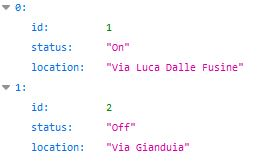
\includegraphics{lamps.jpg}
    \caption{Api risponde a richiesta su /Lamps}
\end{figure}

\begin{figure}[H]
    \centering
    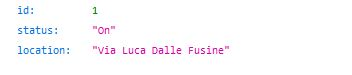
\includegraphics{lampsid.jpg}
    \caption{Api risponde a richiesta su /Lamps/1}
\end{figure}

\subsection{Richiesta PUT}

Come menzionato sopra il progetto offre anche una PUT, anch'essa a Lamps/id. Questo servizio consente di modificare i dettagli della lampadina corrispondente, in particolare di modificare il proprio stato (quindi accenderla o spegnerla).

\begin{figure}[H]
    \centering
    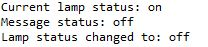
\includegraphics{put1.jpg}
    \caption{Richiesta PUT: La lampadina non è nello stato richiesto}
\end{figure}

\begin{figure}[H]
    \centering
    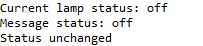
\includegraphics{put2.jpg}
    \caption{Richiesta PUT: La lampadina è già nello stato richiesto}
\end{figure}

\subsection{Comunicazione MQTT}

A ogni richiesta effettuata, l'API posta messaggi sui topic relativi alle lampadine utilizzando mqtt (nel caso del nostro progetto con broker mosquitto), messaggi che vengono successivamente letti dalle nostre applicazioni in back-end. Come spiegato sopra, questo passaggio è essenziale in quanto serve a comunicare con i servizi veri e propri facendogli eseguire le diverse operazioni richieste, tuttavia è più a scopo dimostrativo sul funzionamento della comunicazioni in questo PoC.

\begin{figure}[H]
    \centering
    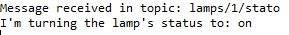
\includegraphics{mqtt.jpg}
    \caption{Richiesta PUT: Client legge il messaggio mqtt in arrivo dall'API}
\end{figure}